\documentclass{article}
\usepackage{amssymb,amsmath,amsthm,bm}
\usepackage{graphicx}
\usepackage{subfigure}
\usepackage{multirow}
\usepackage{wrapfig}
\usepackage[usenames,dvipsnames]{color}
\usepackage{mathrsfs}
\usepackage{enumerate}
\usepackage[bookmarks=true]{hyperref}
\usepackage{bookmark}

\usepackage{amssymb,amsmath,amsthm}
%\newtheorem{mdef}{Definition}
%\newtheorem{theorem}{Theorem}
\newcommand{\eqsplit}[2]{
  \begin{equation}\label{#2}
    \begin{split}
      #1
    \end{split}
  \end{equation}}
\newcommand{\eqnsplit}[1]{
  \begin{eqnarray*}
    #1
  \end{eqnarray*}}
\newcommand{\tran}[1]{
  \tilde{#1}
}
\newcommand{\td}[2]{
  \frac{d #1}{d #2}
}
\newcommand{\pd}[2]{
  \frac{\partial #1}{\partial #2}
}
\newcommand{\ppd}[2]{
  \frac{\partial^2 #1}{\partial #2^2}
}
\newcommand{\pdd}[3]{
  \frac{\partial^2 #1}{\partial #2 \partial #3}
}
\newcommand{\otd}[1]{
  \frac{d}{d #1}
}
\newcommand{\opd}[1]{
  \frac{\partial}{\partial #1}
}
\newcommand{\oppd}[1]{
  \frac{\partial^2}{\partial #1^2}
}
\newcommand{\opdd}[2]{
  \frac{\partial^2}{\partial #1 \partial #2}
}
\newcommand{\ket}[1]{
  |#1\rangle
}
\newcommand{\bra}[1]{
  \langle#1|
}
\newcommand{\inn}[1]{
  \langle#1\rangle
}
\newcommand{\mean}[1]{
  \langle#1\rangle
}
\newcommand{\tr}{
  \text{tr}\,
}
\newcommand{\re}{
  \text{Re}\,
}
\newcommand\im{
  \text{Im}\,
}
\newcommand{\var}{
  \text{var}
}
\newcommand{\arcsinh}{
  \sinh^{-1}
}
\newcommand{\arccosh}{
  \cosh^{-1}
}
\newcommand{\erfc}{
  \text{erfc}
}
\newcommand{\E}{
  \mathbb{E}
}
\renewcommand{\P}{
  \mathbb{P}
}
\newcommand{\I}[1]{
  \mathbf{1}_{\{#1\}}
}
\newcommand{\1}[1]{
  \mathds{1}_{\{#1\}}
}
\newcommand{\diag}{
  \text{diag\,}
}
\newcommand{\M}{
  {\text{max}}
}
\newcommand{\m}{
  {\text{min}}
}
\newcommand{\ph}{
  {\text{arg}\,}
}
\newcommand\erf{
  \text{erf}
}
\renewcommand\vec[1]{
  \mathbf{#1}
}
\newcommand\mtx[1]{
  \mathbf{#1}
}
\newcommand\ed{
  \,{\buildrel d \over =}\,
}



\DeclareGraphicsExtensions{.eps, .pdf}

\author{
  Prof. Sven \AA berg \\
  Xie Xiaolei}
\date{\today}
\title{Effect of Heteroscedasticity in Covariance Matrix}

\begin{document}
\maketitle

\section{Separation of the Heteroscedasticity Effect}
Consider a covariance matrix constructed as
$$
C_{ij} = {1 \over T}\sum_{t=1}^T r_{it} r_{jt}
$$
where $1 \leq i \leq N$. Adopt a stochastic volatility model for
$r_{it}$, i.e.
$$
r_{it} = \sigma_{it} \eta_{it}
$$
We can write
\begin{eqnarray}
C_{ij} &=& {1 \over T}\sum_{t=1}^T \sigma_{it} \eta_{it} \sigma_{jt}
\eta_{jt} \nonumber \\
\bm{C} &=& {1 \over T} (\bm{\sigma * \eta}) (\bm{\sigma *
  \eta})' \label{eq:C}
\end{eqnarray}
where the matrices $\bm{\sigma}$ and $\bm{\eta}$ have elements
$\sigma_{it}$ and $\eta_{it}$ respectively, and * denotes element-wise
multiplication. Due to the cyclic property of matrix trace, the
moment generating function of $\bm{C}$, $M_C(z)$, relates to $M_D(z)$,
the moment generating function of $\bm D$
\begin{eqnarray*}
  \bm{D} &=& {1 \over T} (\bm{\sigma * \eta})' (\bm{\sigma * \eta})
\end{eqnarray*}
through the equation
\begin{eqnarray*}
  M_C(z) &=& {1 \over q} M_D(z)
\end{eqnarray*}
where $q = N/T$. For later convenience, we make use of $T \times T$
matrices $\bm{\tilde{\sigma}}$ and $\bm{\tilde{\eta}}$, as well as a
projector
$$
\bm{P} = \text{diag}(\underbrace{1, \cdots, 1}_{\text{N 1's}}, 
\underbrace{0, \cdots, 0}_{\text{T-N 0's}})
$$
The first N rows of $\tilde{\bm{\sigma}}$ and $\bm{\tilde{\eta}}$ are
precisely those of $\bm{\sigma}$ and $\bm{\eta}$. This way, we have
\begin{eqnarray*}
\bm D &=& {1 \over T} (\bm{\sigma * \eta})' (\bm{\sigma * \eta}) \\
&=& {1 \over T} (\bm{\tilde{\sigma} * \tilde{\eta}})' \bm P'
\bm P (\bm{\tilde{\sigma} * \tilde{\eta}}) \\
&=& {1 \over T} (\bm{\tilde{\sigma} * \tilde{\eta}})'
\bm P (\bm{\tilde{\sigma} * \tilde{\eta}}) \\
\end{eqnarray*}
Again, by the cyclic property of matrix trace, the spectral properties
of the RHS of the last equation is equivalent to those of
\begin{eqnarray*}
  \bm E &=& {1 \over T} (\bm{\tilde{\sigma} * \tilde{\eta}}) (\bm{\tilde{\sigma}
    * \tilde{\eta}})' \bm P \\
\end{eqnarray*}
In the simple situation where $\sigma_{it} =
\sigma_{jt} = \sigma_t$ for some $\sigma_t$ and for all $i, j, t$,
\begin{eqnarray*}
  \bm{\tilde \sigma * \tilde \eta} &=& \bm{\tilde \eta}
  \begin{pmatrix}
    \sigma_1 &        & \\
        & \ddots & \\
        &        & \sigma_T
  \end{pmatrix} \\
  &=& \bm{\tilde \eta \bar \sigma}
\end{eqnarray*}
Thus
\begin{eqnarray}\label{eq:E_def}
  \bm E &=& {1 \over T}\bm{\tilde \eta \bar \sigma^2 \tilde \eta' P}
\end{eqnarray}
In the large T limit $\bm{\tilde \eta \bar \sigma^2 \tilde \eta'}$ and $P$ are
freely independent, therefore their S-transforms are multiplicative,
i.e.
\begin{eqnarray}
  S_E(z) &=& S_{\tilde \eta \bar \sigma^2 \tilde \eta'/T}(z) S_P(z)
  \nonumber \\
  &=& S_{\tilde \eta' \tilde \eta /T}(z) S_{\bar \sigma^2}(z) S_P(z) \label{eq:S_E}
\end{eqnarray}
For $S_{\tilde \eta' \tilde \eta /T}(z)$ there have been results when
the elements of $\bm{\tilde \eta}$ are identically distributed with finite
second moment \cite{burda2011} or alternatively, follow $\alpha$-stable
distribution \cite{politi2010}.

So our focus hereafter is on the spectral properties of $\bar{
\bm \sigma^2}$. The Green's function of $\bar{\bm \sigma^2}$
can be immediately written down:
\begin{eqnarray*}
G_{\bar \sigma^2} &=& \frac{1}{T}\sum_{t=1}^T \frac{1}{z - \sigma_t^2}
\end{eqnarray*}
Suppose the $\sigma_t^2$ process has correlation time $\tau$,
i.e. $\text{corr}(\sigma_t^2, \sigma^2_{t+\tau}) \approx 0$. Then we
have
\begin{eqnarray*}
G_{\bar \sigma^2} &=& {1 \over T}\sum_{n=0}^{\tau-1}\sum_{m=1}^{T/\tau}
\frac{1}{z - \sigma_{m\tau + n}^2} \\
&=& {1 \over \tau}\sum_{n=0}^{\tau-1} {1 \over T/\tau}
\sum_{m=1}^{T/\tau} \frac{1}{z - \sigma_{m\tau + n}^2} \\
&=& {1 \over \tau}\sum_{n=0}^{\tau-1}
\E_m\left(\frac{1}{z - \sigma_{m\tau + n}^2}\right)
\end{eqnarray*}
where $\E_m$ denotes averaging over the index $m$. On condition that
$\sigma_t^2$ is a stationary process, $\E_m[1 / (z -
    \sigma_{m\tau + n}^2)]$ is independent of $n$. Thus
\begin{eqnarray}\label{eq:greens}
G_{\bar \sigma^2} &=& \E_m\left(
  \frac{1}{z - \sigma_{m\tau + n}^2}
\right)
\end{eqnarray}
So autocorrelations of $\sigma_t^2$'s affect spectral properties
only through the stationary distribution of $\sigma_t^2$.
In the following subsections we discuss situations where $\sigma_t$'s
are chosen from different conditional distributions and have different
autocorrelation structures.
% Then the moment generating function $M_{\bar \sigma^2}$ is
% \begin{eqnarray*}
%   M_{\bar \sigma^2} &=& z G_{\bar \sigma^2} - 1 \\
%   &=& \frac{1}{T} \sum_{t=1}^T \frac{1}{1 - \sigma_t^2/z} - 1\\
%   &=& \frac{1}{T} \sum_{n=0}^{\infty} \frac{1}{z^n}\sum_{t=1}^T
%   \sigma_t^{2n} - 1\\
%   &=& \frac{1}{T} \sum_{n=1}^{\infty} \frac{1}{z^n}\sum_{t=1}^T
%   \sigma_t^{2n}
% \end{eqnarray*}

\section{Normal innovations \& log-normal volatilities with AR(1)
  autocorrelation}
In this subsection we consider the case
\begin{eqnarray}
  \log \sigma_t &=& \phi\log \sigma_{t-1} + x_t \nonumber \\
  &=& \sum_{l = 0}^{\infty} \phi^l x_{t-l} \label{eq:AR}
\end{eqnarray}
where $x_t \sim N(0, 1)$ and we have assumed that the $\log \sigma_t$
process was started in the infinite past with $\log \sigma_{-\infty} =
x_{-\infty}$. In addition, we assume $\log \sigma_t$ is a stationary
process with $|\phi| < 1$. Clearly $\log \sigma_t$ is normally
distributed with mean 0 and variance ${1 / (1 -
  \phi^2)}$. According to \eqref{eq:greens}, the spectral density of
$\bm E$ as appears in \eqref{eq:E_def} is the same as if
$\sigma_t^2$'s were uncorrelated but $\log \sigma_t \sim N(0,
1/(1 - \phi^2))$.

To find the spectral density of $\bm C$ with normally distributed $\bm
\eta$ and uncorrelated, log-normally distributed $\sigma_t$, we use
the result of Biroli et al in \cite{biroli2007student}, which gives
the Blue function of $\bm C$ as
\begin{eqnarray*}
  B(z) &=& \frac{1}{z} + \int \frac{\sigma ^2 P(s) ds}{1-q \sigma ^2 z}
\end{eqnarray*}
where $q = N/T$ and $\sigma$ has the stationary distribution of
$\sigma_t$, whose probability density function is $P(s)$. Now we are
specifically considering lognormally distributed $\sigma_t$, so we
rewrite the above equation as
\begin{eqnarray}
B(z) &=& \int_{-\infty }^{\infty } \frac{e^{2 s} \exp \left(-\frac{s^2}{2
      v}\right)}{\sqrt{2 \pi  v} \left(1-q e^{2 s} z\right)} \,
ds+\frac{1}{z} \label{eq:LognormalBlue}
\end{eqnarray}
where $v = 1/(1 - \phi^2)$, reflecting the effect
of autocorrelation in $\log \sigma_t$'s. However, no closed form of
this integral is known to the author. To obtain the spectral density,
which is given by the Sokhotski-Weierstrass formula as
\begin{eqnarray}
  \rho(\lambda) &=& -{1 \over \pi} \lim_{\epsilon \to 0} \im G(\lambda +
  i\epsilon) \label{eq:Sokhotski-Weierstrass}
\end{eqnarray}
we equate the real part of RHS of \eqref{eq:LognormalBlue} to $\lambda \in
R$ and the imaginery part to 0, then we can solve \eqref{eq:LognormalBlue}
numerically and obtain $\rho(\lambda)$ via
\eqref{eq:Sokhotski-Weierstrass}. Specifically we solve the following
equation system:
\begin{eqnarray}
\lambda &=& \int_{-\infty}^{\infty} \frac{ds}{\sqrt{2\pi v}}
\frac{
  e^{-s^2/2v}(e^{-2s} - qx)
}{
  (e^{-2s} - qx)^2 + q^2 y^2  
} +
\frac{x}{x^2 + y^2} \label{eq:LognormalBlueReal}\\
0 &=& \int_{-\infty}^{\infty} \frac{ds}{\sqrt{2\pi v}}
\frac{
  e^{-s^2/2v} q y
}{
  (e^{-2s} - qx)^2 + q^2 y^2  
} -
\frac{y}{x^2 + y^2} \label{eq:LognormalBlueImag}
\end{eqnarray}
This is the method used by Biroli et al in
\cite{biroli2007student}. Figure \ref{fig:LognormalBlue}
shows the plot of the Blue function \eqref{eq:LognormalBlue}. $-\pi
\rho(\lambda)$ is the projection of the contour $\im B(z) = 0$ onto the $\im
G$ axis.
\begin{figure}[htb!]
  \centering
    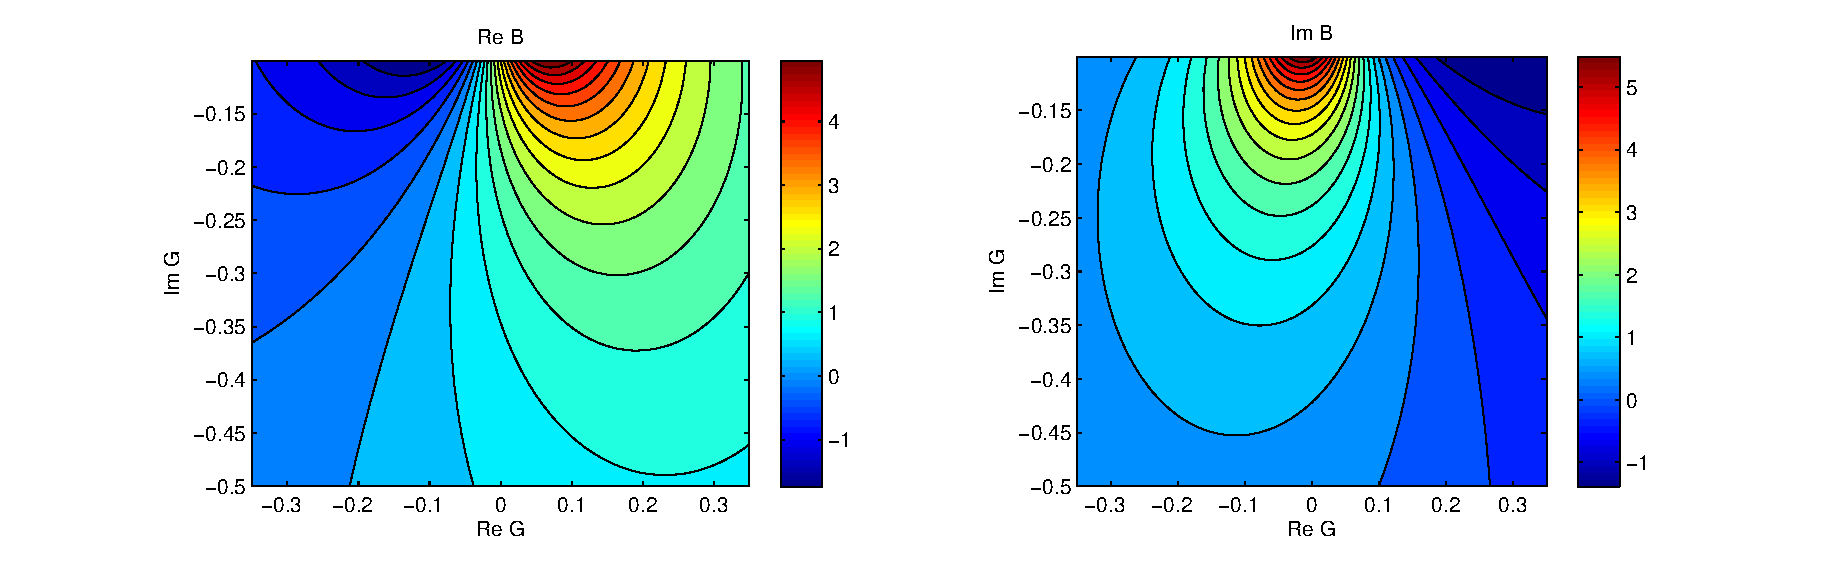
\includegraphics[scale=0.45, clip=true, trim=66 0 84
    0]{../pics/LognormalBlue.eps}
  \caption{\small \it The Blue function $B$. q = 0.45, v = 3}
  \label{fig:LognormalBlue}
\end{figure}
The spectral density function $\rho(\lambda)$ obtained as numerical
solutions is shown in figure \ref{fig:LognormalSpectra} and compared
to the Marcenko-Pastur law with several values of $q = N/T$ and $v$.
\begin{figure}[htb!]
  \centering
  \subfigure[$q = 0.1$]{
    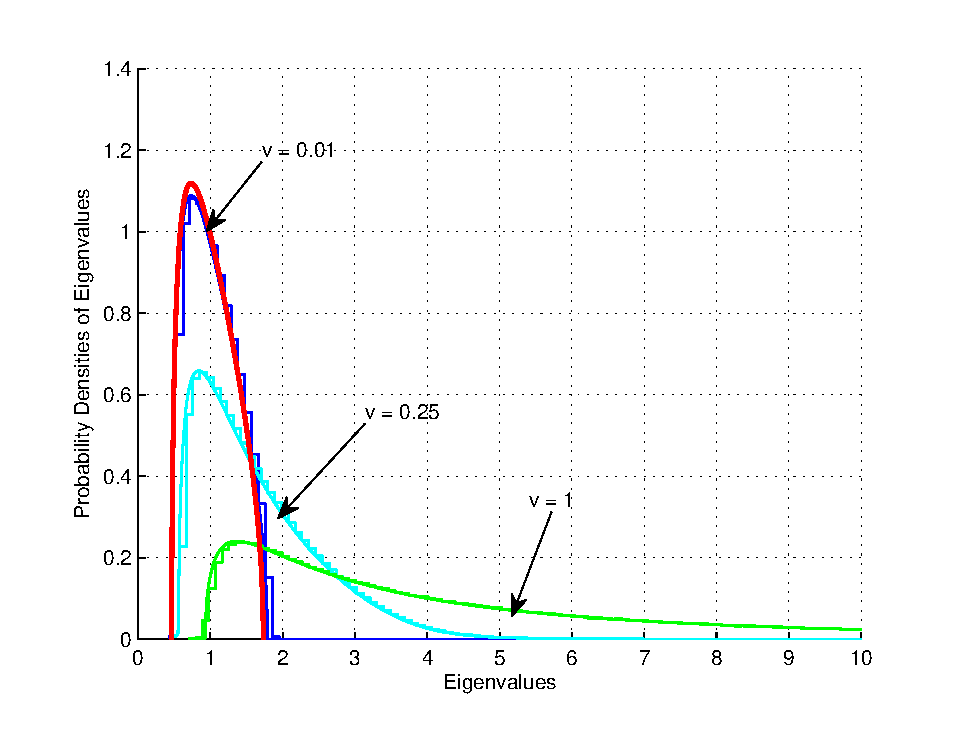
\includegraphics[scale=0.35]{../pics/Lognormal_q0.1.eps}
    \label{fig:Lognormal_q0.1}
  }
  \subfigure[$q = 0.2$]{
    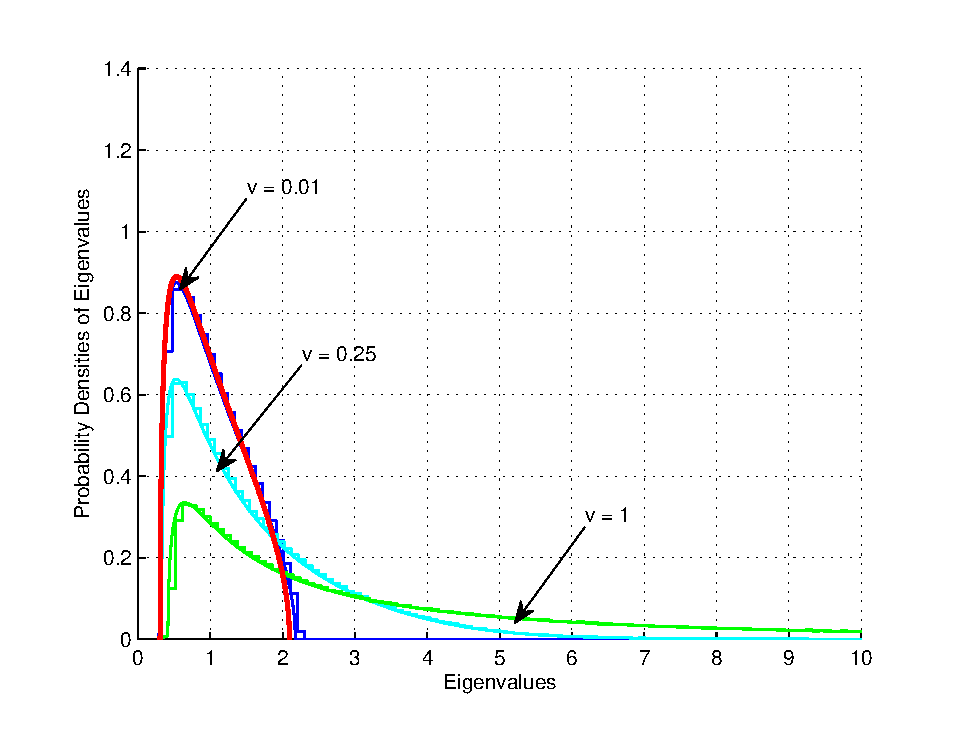
\includegraphics[scale=0.35]{../pics/Lognormal_q0.2.eps}
    \label{fig:Lognormal_q0.2}
  }
  \subfigure[$q = 0.5$]{
    \includegraphics[scale=0.35]{../pics/Lognormal_q0.5.eps}
    \label{fig:Lognormal_q0.5}
  }
  \subfigure[$q = 1.0$]{
    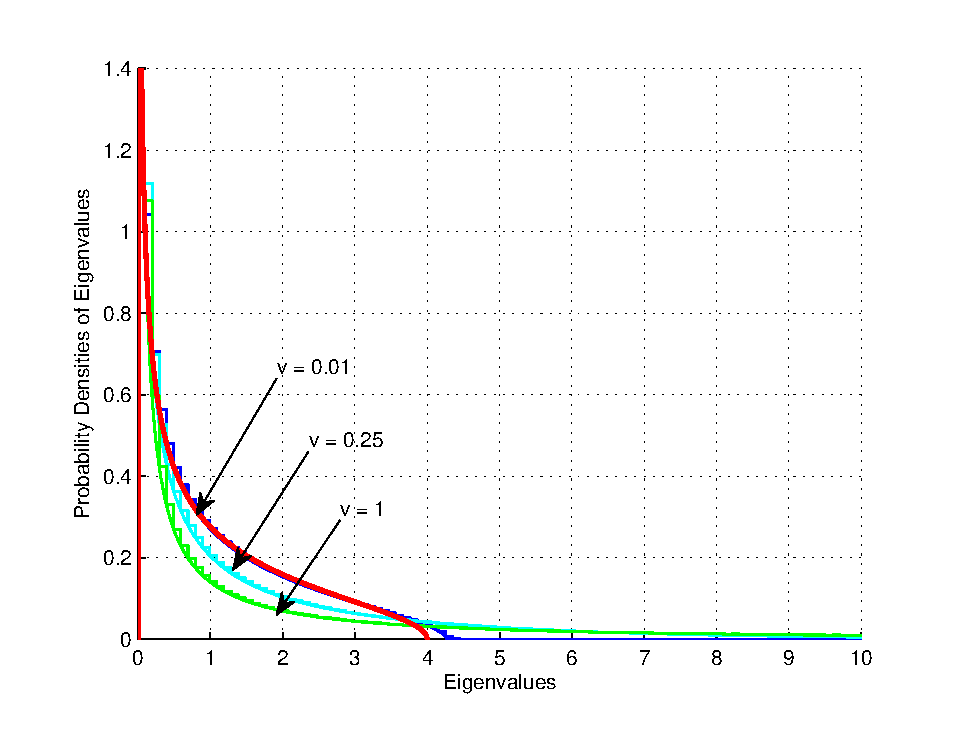
\includegraphics[scale=0.35]{../pics/Lognormal_q1.0.eps}
    \label{fig:Lognormal_q1.0}
  }
  % \subfigure[$v=1$, $q = 1$]{
  %   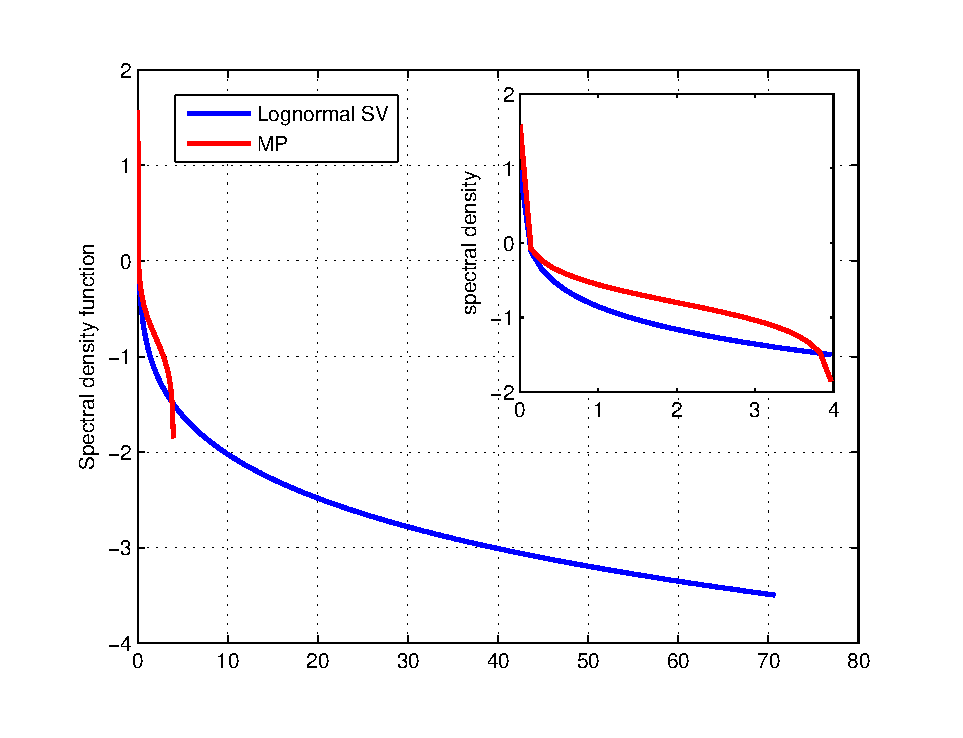
\includegraphics[scale=0.35]{../pics/Lognormal_v1_q1.eps}
  %   \label{fig:Lognormal_v1_q1}
  % }
  % \subfigure[$v=1$, $q = 0.1$]{
  %   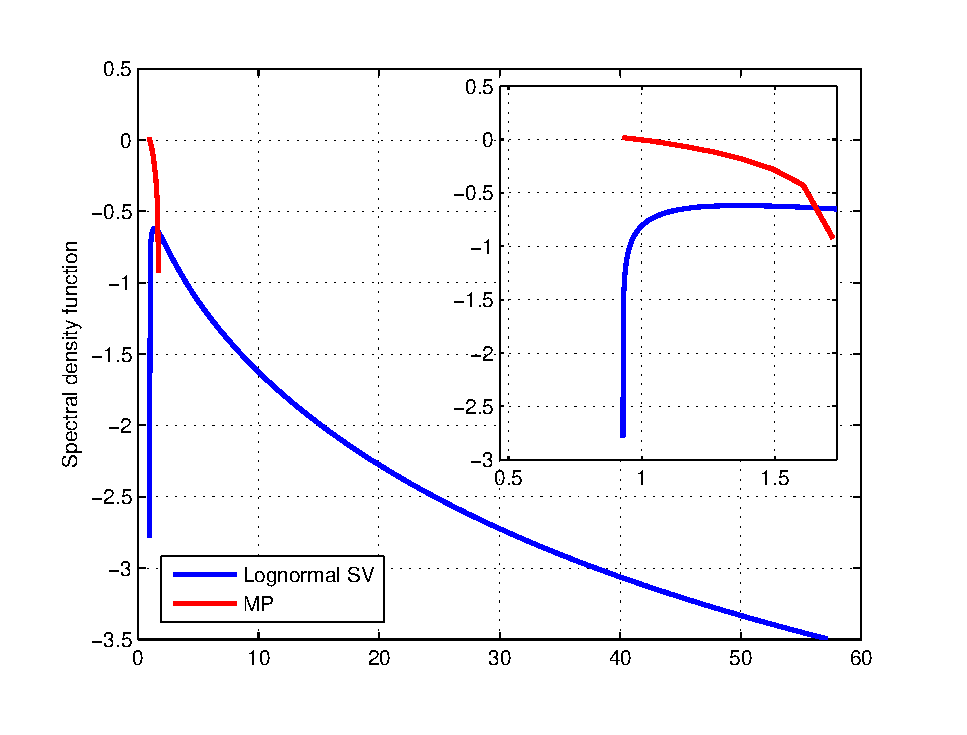
\includegraphics[scale=0.35]{../pics/Lognormal_v1_q0.1.eps}
  %   \label{fig:Lognormal_v1_q0.1}
  % }
  % \subfigure[$v=0.0001$, $q = 1$]{
  %   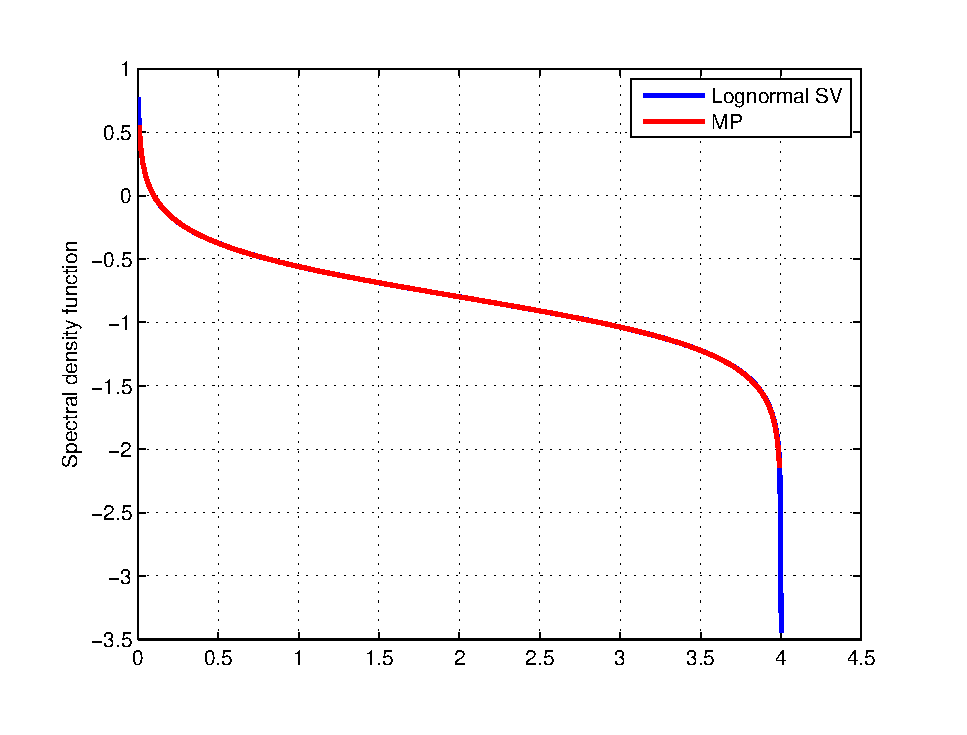
\includegraphics[scale=0.35]{../pics/Lognormal_v0.0001_q1.eps}
  %   \label{fig:Lognormal_v0.0001_q1}
  % }
  % \subfigure[$v=0.0001$, $q = 0.1$]{
  %   \includegraphics[scale=0.35]{../pics/Lognormal_v0.0001_q0.1.eps}
  %   \label{fig:Lognormal_v0.0001_q0.1}
  % }
  \caption{\small \it Spectra with lognormal volatilities. The
    empirical probability density functions are plotted as stairs. The
  density function given by the Marcenko-Pastur law is plotted as a
  thick red curve.}
  \label{fig:LognormalSpectra}
\end{figure}
From figures \ref{fig:LognormalSpectra} one can see that the
Marcenko-Pastur law is recovered when $v \to 0$, as expected.

Now we consider equation \eqref{eq:LognormalBlueReal} and
\eqref{eq:LognormalBlueImag}. When $q y$ and $v$ are both small, RHS
of \eqref{eq:LognormalBlueReal} and \eqref{eq:LognormalBlueImag} have
two sharp peaks, one at $s = 0$ and the other at $s = -{1 \over
  2}\ln(qx)$. We expand the integrands in
\eqref{eq:LognormalBlueReal} and \eqref{eq:LognormalBlueImag} around
these two peaks. For \eqref{eq:LognormalBlueImag} We write
\begin{eqnarray}
  {y \over x^2 + y^2} &=& \int_{-a}^{a} {e^{-s^2/2v}ds \over
    \sqrt{2\pi v}} \left[\frac{qy}{(1-qx)^2 + q^2y^2}\right] \label{eq:lambda}\\
  && - \int_{-b}^{b} {dt \over \sqrt{2\pi v}} {1 \over 2(t + q x)}
  \exp \left[-\frac{\log ^2(q x+t)}{8v}\right] {qy \over t^2 +
    q^2y^2} \nonumber \\
  &=& \erf\left({a \over \sqrt{2\pi}}\right)\left[\frac{qy}{(1-qx)^2 +
      q^2 y^2}\right] \nonumber \\
  && -{1 \over \sqrt{2\pi v}}\left\{
  \exp\left(-{\ln^2qx \over 8v}\right) \frac{x \cot ^{-1}\left(\frac{q
      y}{b}\right)+y \coth ^{-1}\left(\frac{q x}{b}\right)}{q x^2+q
    y^2} \right. \nonumber \\
  && \left.-\exp\left(-{\ln^2qx \over 8v}\right)
  \frac{y \left[x \log \left(1-\frac{2 b}{b+q x}\right)+2 y
    \cot^{-1}\left(\frac{q y}{b}\right)\right]}{2
    \left(x^2+y^2\right)} {\ln qx \over 4qvx}
  \right\} \nonumber
\end{eqnarray}
where $a$ and $b$ are small positive numbers. In particular, $b < q x$
such that $t + qx > 0$. Similarly, for \eqref{eq:LognormalBlueReal} we have
\begin{eqnarray}
  \lambda &=& {x \over x^2 + y^2} + \erf\left({a \over \sqrt{2v}}\right){1 - q x
    \over (1 - q x)^2 + q^2 y^2 } \nonumber \\
  && - {1 \over \sqrt{2\pi v}}
  \left\{\exp\left(-{\ln^2qx \over 8v}\right) \frac{x \log
    \left(1-\frac{2 b}{b+q x}\right)+2 y \cot ^{-1}\left(\frac{q
      y}{b}\right)}{2 q \left(x^2+y^2\right)} \right. \nonumber \\
  &&  
  \left. -\frac{\log (q x)}{4 q v x} \exp\left(-{\ln^2qx \over
    8v}\right) \frac{x \left[x \coth ^{-1}\left(\frac{q x}{b}\right)-y
    \cot ^{-1}\left(\frac{q y}{b}\right)\right]}{x^2+y^2}
  \right\} \label{eq:constraint}
\end{eqnarray}
%% Now we consider equation \eqref{eq:LognormalBlueReal} and
%% \eqref{eq:LognormalBlueImag}. As $\lambda$ tends to $\lambda_\M$ with
%% $\lambda_\M \leq \infty$, $y \to 0$. Meanwhile, $x$ can neither tend
%% to 0 nor to $\infty$: If $x \to 0$, then $\frac{1}{x^2 + y^2} \to
%% \infty$ while the integral in \eqref{eq:LognormalBlueImag} tends to
%% $e^{8v}$ -- thus \eqref{eq:LognormalBlueImag} cannot hold. If instead
%% $x \to \infty$, RHS of \eqref{eq:LognormalBlueReal} tends to 0, failing
%% \eqref{eq:LognormalBlueReal}. So $x$ must tend to a finite value as $\lambda
%% \to \lambda_\M$. This limiting value, call it $a$, can be found from
%% \eqref{eq:LognormalBlueImag} by setting $y=0$:
%% \begin{eqnarray}
%% {1 \over a^2} &=& \int_{-\infty}^{\infty} \frac{ds}{\sqrt{2\pi v}}
%% \frac{
%%   e^{-s^2/2v} q
%% }{
%%   (e^{-2s} - qa)^2
%% } \label{eq:LognormalBlueImag2}
%% \end{eqnarray}
%% Clearly $a$ is a function of $v$ and $q$. Denote this function $f$
%% such that $a = f(v, q)$. As has been argued, $f(v,q)$ is finite for
%% all $v > 0$ and $0 < q \leq 1$. Using $f$, the integral in
%% \eqref{eq:LognormalBlueReal}, in the limit $\lambda \to \lambda_\M$,
%% can be expressed
%% \begin{eqnarray*}
%%   {1 \over \sqrt{2\pi v}} \int_{-\infty}^{\infty} \frac{
%%     e^{-2s - s^2/2v}
%%     }{
%%       (e^{-2s} - qa)^2
%%     } ds &=& {1 \over q e^{2v} f^2(v, qe^{-4v})}
%% \end{eqnarray*}
%% It immediately follows from \eqref{eq:LognormalBlueReal}
%% \begin{eqnarray*}
%%   \lambda_\M &=& {1 \over q e^{2v} f^2(v, qe^{-4v})}
%% \end{eqnarray*}
%% Since $q \leq 1$ and $e^{-2v} < 1$, $f(v, qe^{-2v})$ and hence
%% $\lambda_\M$ are finite. The spectrum is bounded.

%% The function $f(v,q)$ as defined by the largest root of
%% \eqref{eq:LognormalBlueImag2} is plotted in figure
%% \ref{fig:FFunction1}, seen as the intersection between the two curves,
%% which represent the two sides of \eqref{eq:LognormalBlueImag2},
%% respectively.
%% \begin{figure}[htb!]
%%   \centering
%%   \subfigure[]{
%%     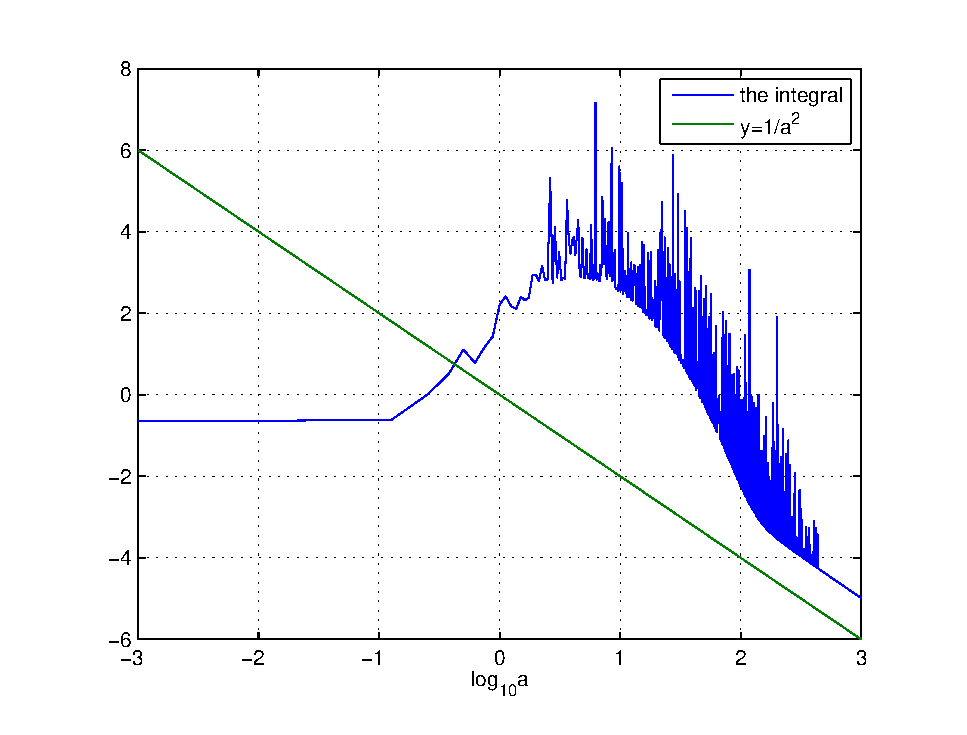
\includegraphics[scale=0.35]{../pics/FFunctionOverview.eps}
%%     \label{fig:FFunctionOverview}
%%   }
%%   \subfigure[]{
%%     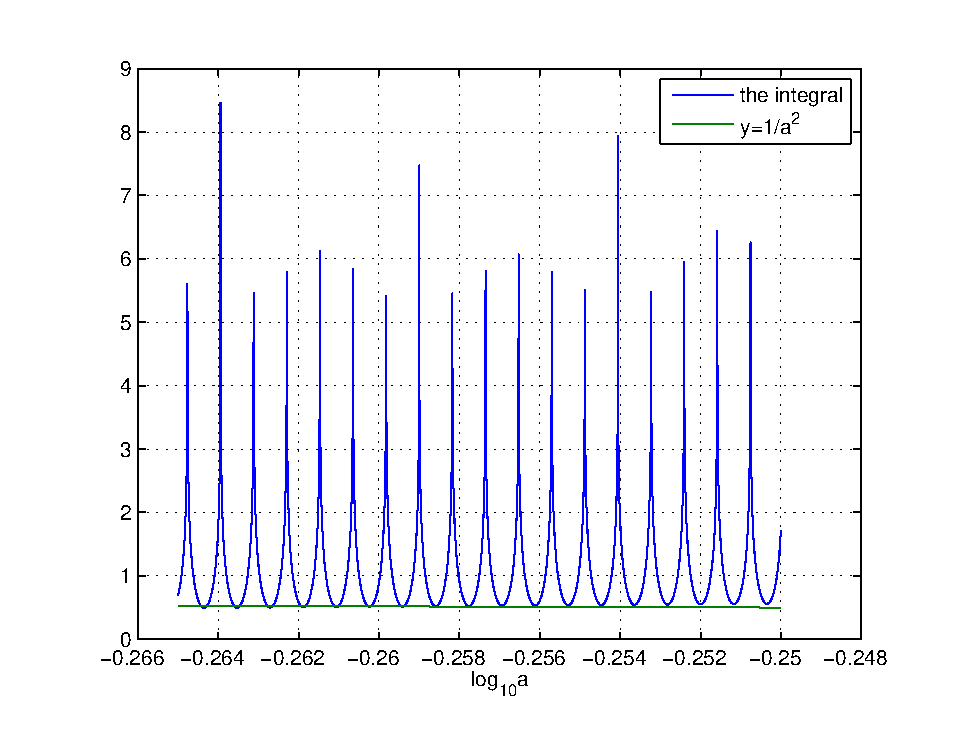
\includegraphics[scale=0.35]{../pics/FFunction1.eps}
%%     \label{fig:FFunction1}
%%   }
%%   %% \subfigure[$q = 0.5$]{
%%   %%   \includegraphics[scale=0.35]{../pics/FFunction3.eps}
%%   %%   \label{fig:FFunction2}
%%   %% }
%%   \caption{\small \it The implicit function $f(v, q)$ plotted in
%%     log-log scale. Blue: the integral $\int_{-\infty}^{\infty}
%%     \frac{ds}{\sqrt{2\pi v}}
%%     \frac{
%%       e^{-s^2/2v} q
%%     }{
%%       (e^{-2s} - qa)^2
%%     }$as a function of $a$. Green: the function $1/a^2$. v=0.1, q=0.1.
%% }
%%   \label{fig:FFunction}
%% \end{figure}

% To see the effect of heteroscedasticity we turn to simulations. Figure
% \ref{fig:LognormalSpectraAutocorrelated} shows the empirical spectral
% density when the conditional log-volatilities are given by \eqref{eq:AR}.
% \begin{figure}[htb!]
%   \centering
%   \subfigure[$q = 0.1$, $\text{var}(x_t) = 0.01$,
%   $\phi = 0$, $\text{var}(\ln\sigma_t) = 0.01$]{
%     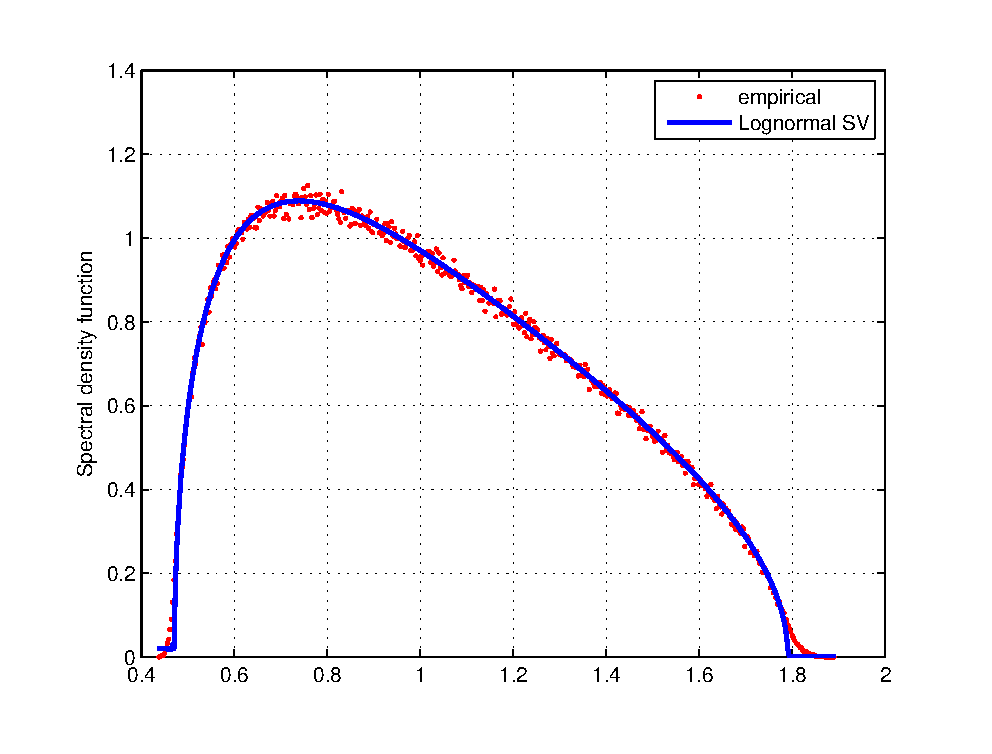
\includegraphics[scale=0.23]{../pics/Lognormal_sig0.1_phi0.eps}
%     \label{fig:Lognormal_sig0.1_phi_0}
%   }
%   \subfigure[$q = 0.1$, $\text{var}(x_t) = 0.01$,
%   $\phi = 0.25$, $\text{var}(\ln\sigma_t) = 0.0107$]{
%     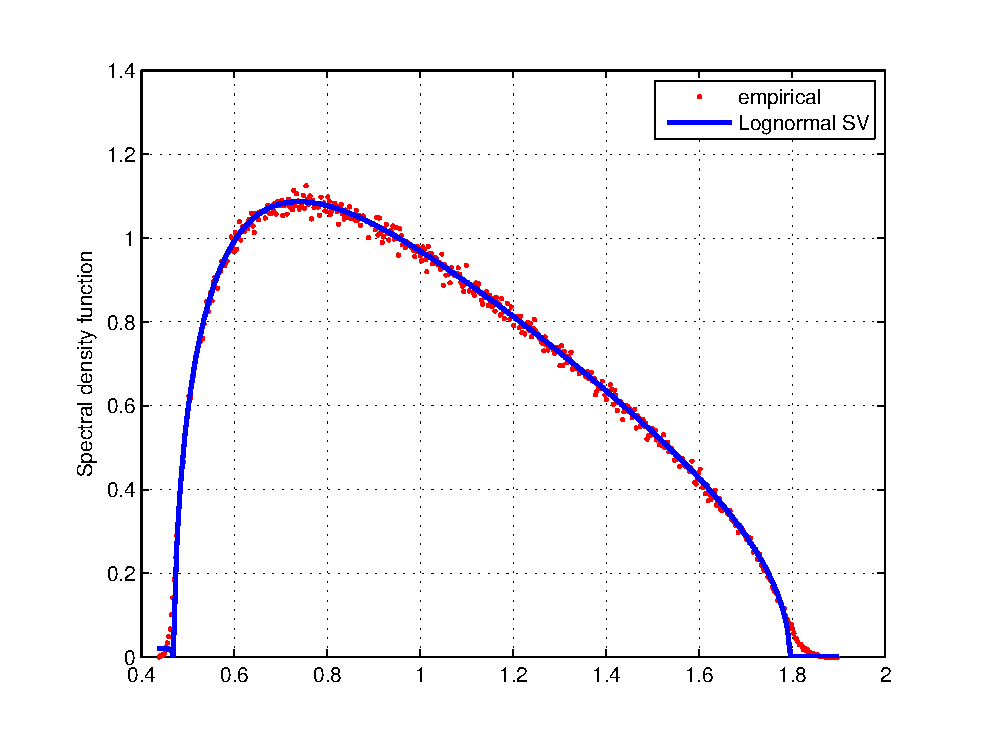
\includegraphics[scale=0.23]{../pics/Lognormal_sig0.1_phi0.25.eps}
%     \label{fig:Lognormal_sig0.1_phi_0.25}
%   }
%   \subfigure[$q = 0.1$, $\text{var}(x_t) = 0.01$,
%   $\phi = 0.5$, $\text{var}(\ln\sigma_t) = 0.0133$]{
%     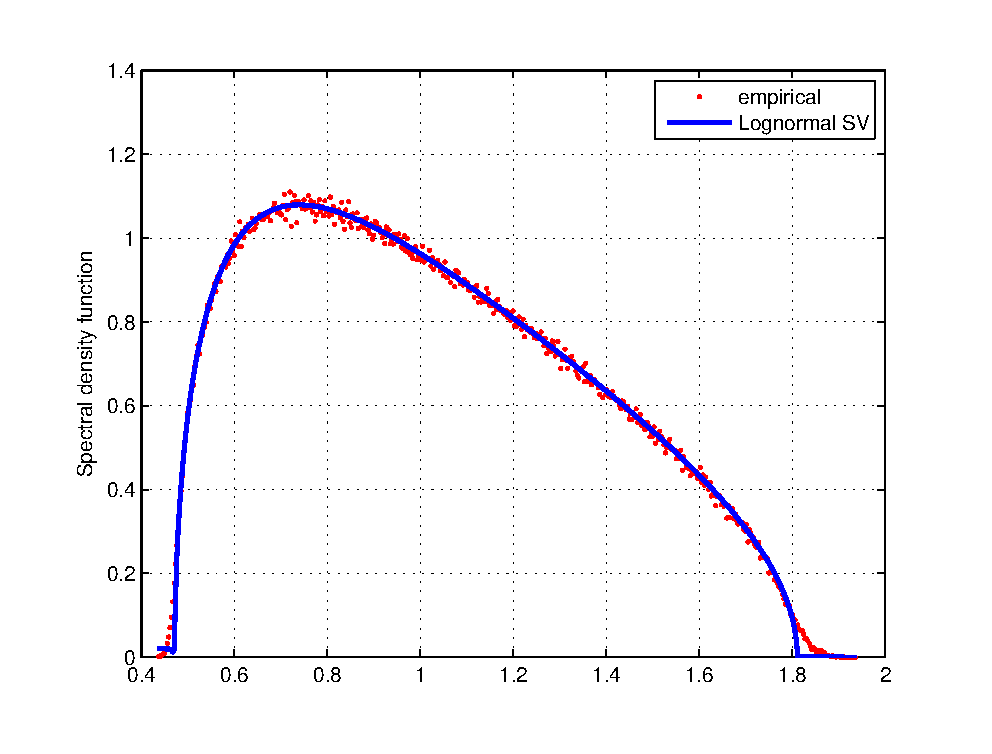
\includegraphics[scale=0.23]{../pics/Lognormal_sig0.1_phi0.5.eps}
%     \label{fig:Lognormal_sig0.1_phi_0.5}
%   }
%   \subfigure[$q = 0.1$, $\text{var}(x_t) = 0.25$,
%   $\phi = 0$, $\text{var}(\ln\sigma_t) = 0.25$]{
%     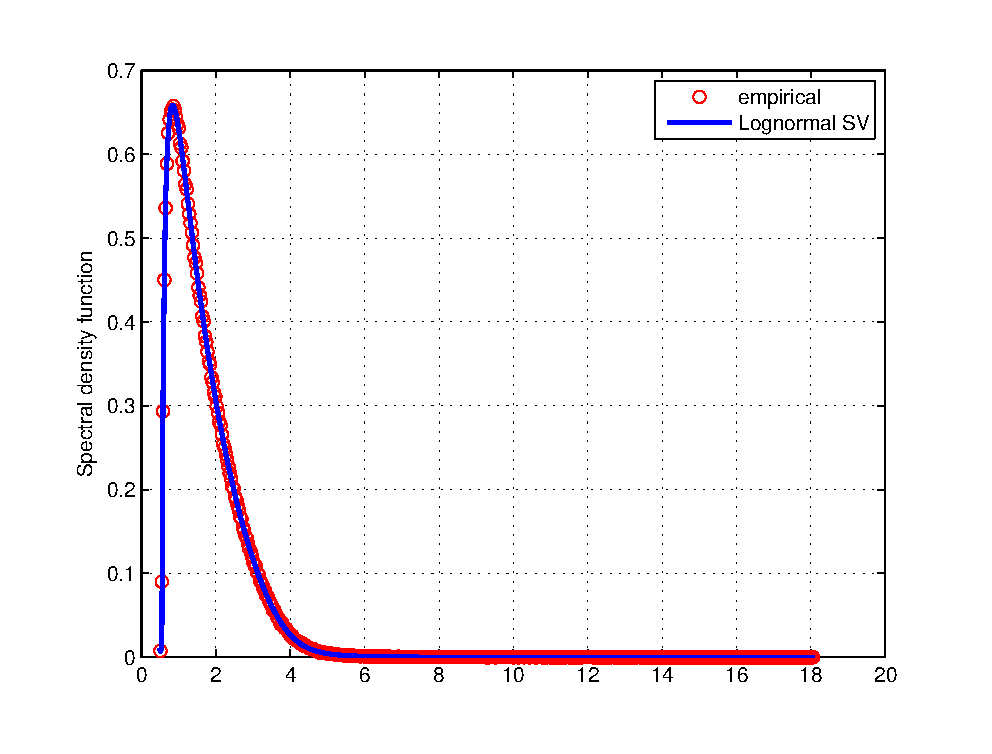
\includegraphics[scale=0.23]{../pics/Lognormal_sig0.5_phi0.eps}
%     \label{fig:Lognormal_sig0.5_phi_0}
%   }
%   \subfigure[$q = 0.1$, $\text{var}(x_t) = 0.25$,
%   $\phi = 0.25$, $\text{var}(\ln\sigma_t) = 0.2667$]{
%     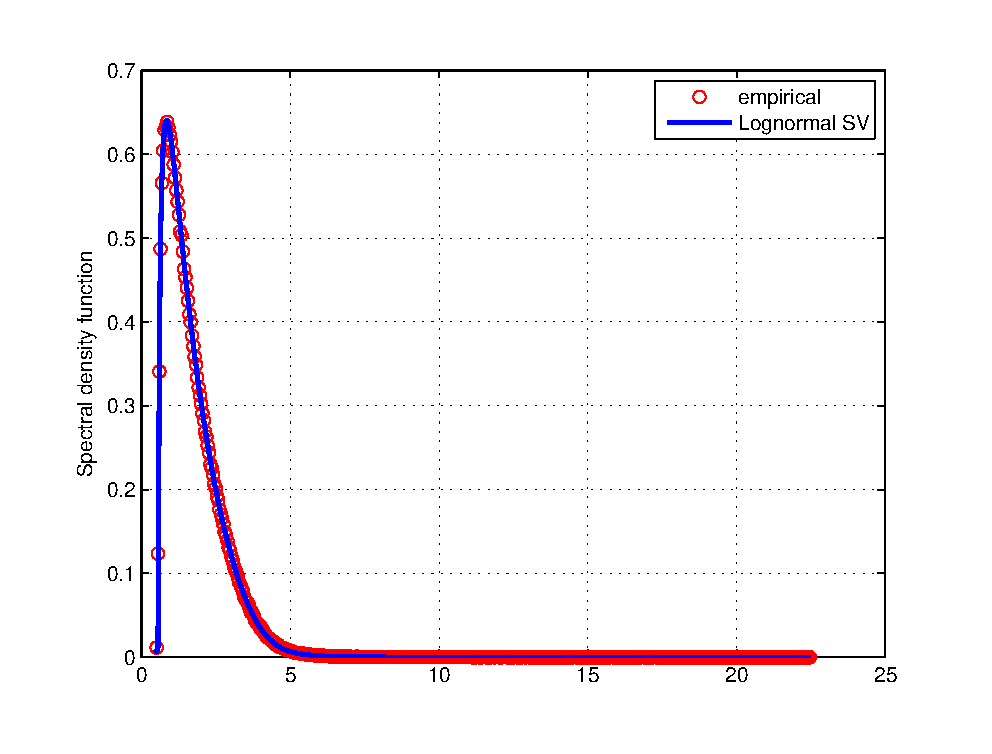
\includegraphics[scale=0.23]{../pics/Lognormal_sig0.5_phi0.25.eps}
%     \label{fig:Lognormal_sig0.5_phi_0.25}
%   }
%   \subfigure[$q = 0.1$, $\text{var}(x_t) = 0.25$,
%   $\phi = 0.5$, $\text{var}(\ln\sigma_t) = 0.3333$]{
%     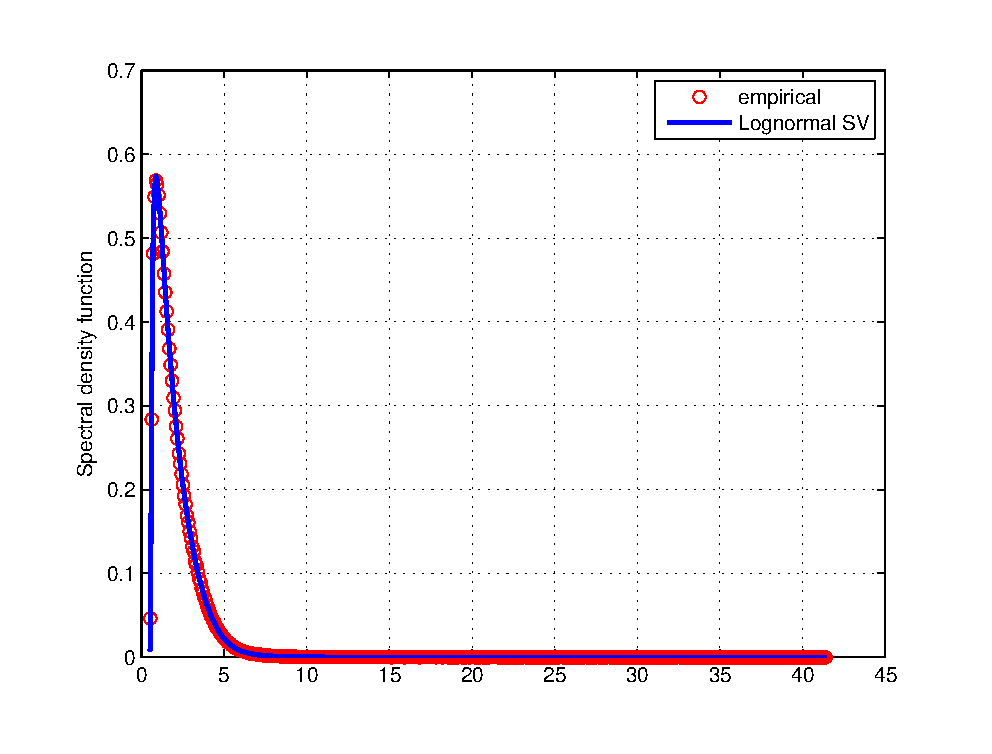
\includegraphics[scale=0.23]{../pics/Lognormal_sig0.5_phi0.5.eps}
%     \label{fig:Lognormal_sig0.5_phi_0.5}
%   }
%   \caption{\small \it Spectra with autocorrelated normal log-volatilities.}
%   \label{fig:LognormalSpectraAutocorrelated}
% \end{figure}
% It is seen that the empirical spectral density agrees very well with
% the density function obtained as numerical solutions to $B(\re G -
% i\pi\rho) = \lambda$.

\bibliographystyle{unsrt}
\bibliography{econophysics}
\end{document}
